\subsection{Use case beskrivelser}
\begin{itemize}
	\item Spil spillet.
	
Spilleren spiller spillet.
\end{itemize}
Sub use case beskrivelser:
\begin{itemize}
	\item Indtast navn.\\ Spilleren indtaster sit navn.
	\item Vælg farve. \\ Spilleren vælger imellem et udvalg af farve.
	\item Rul terning. \\ Spilleren ruller med terningerne.
\end{itemize}

\subsection{Fully dressed Use case}
\begin{figure}[h!]
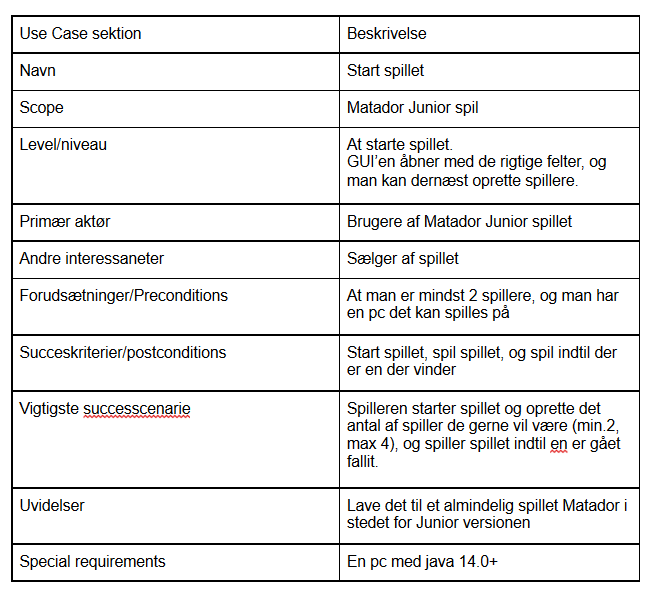
\includegraphics[scale=1]{artifacts/fullyDressed.png}
\end{figure}
\newpage
\subsection{Systemsekvensdiagram}
\begin{figure}
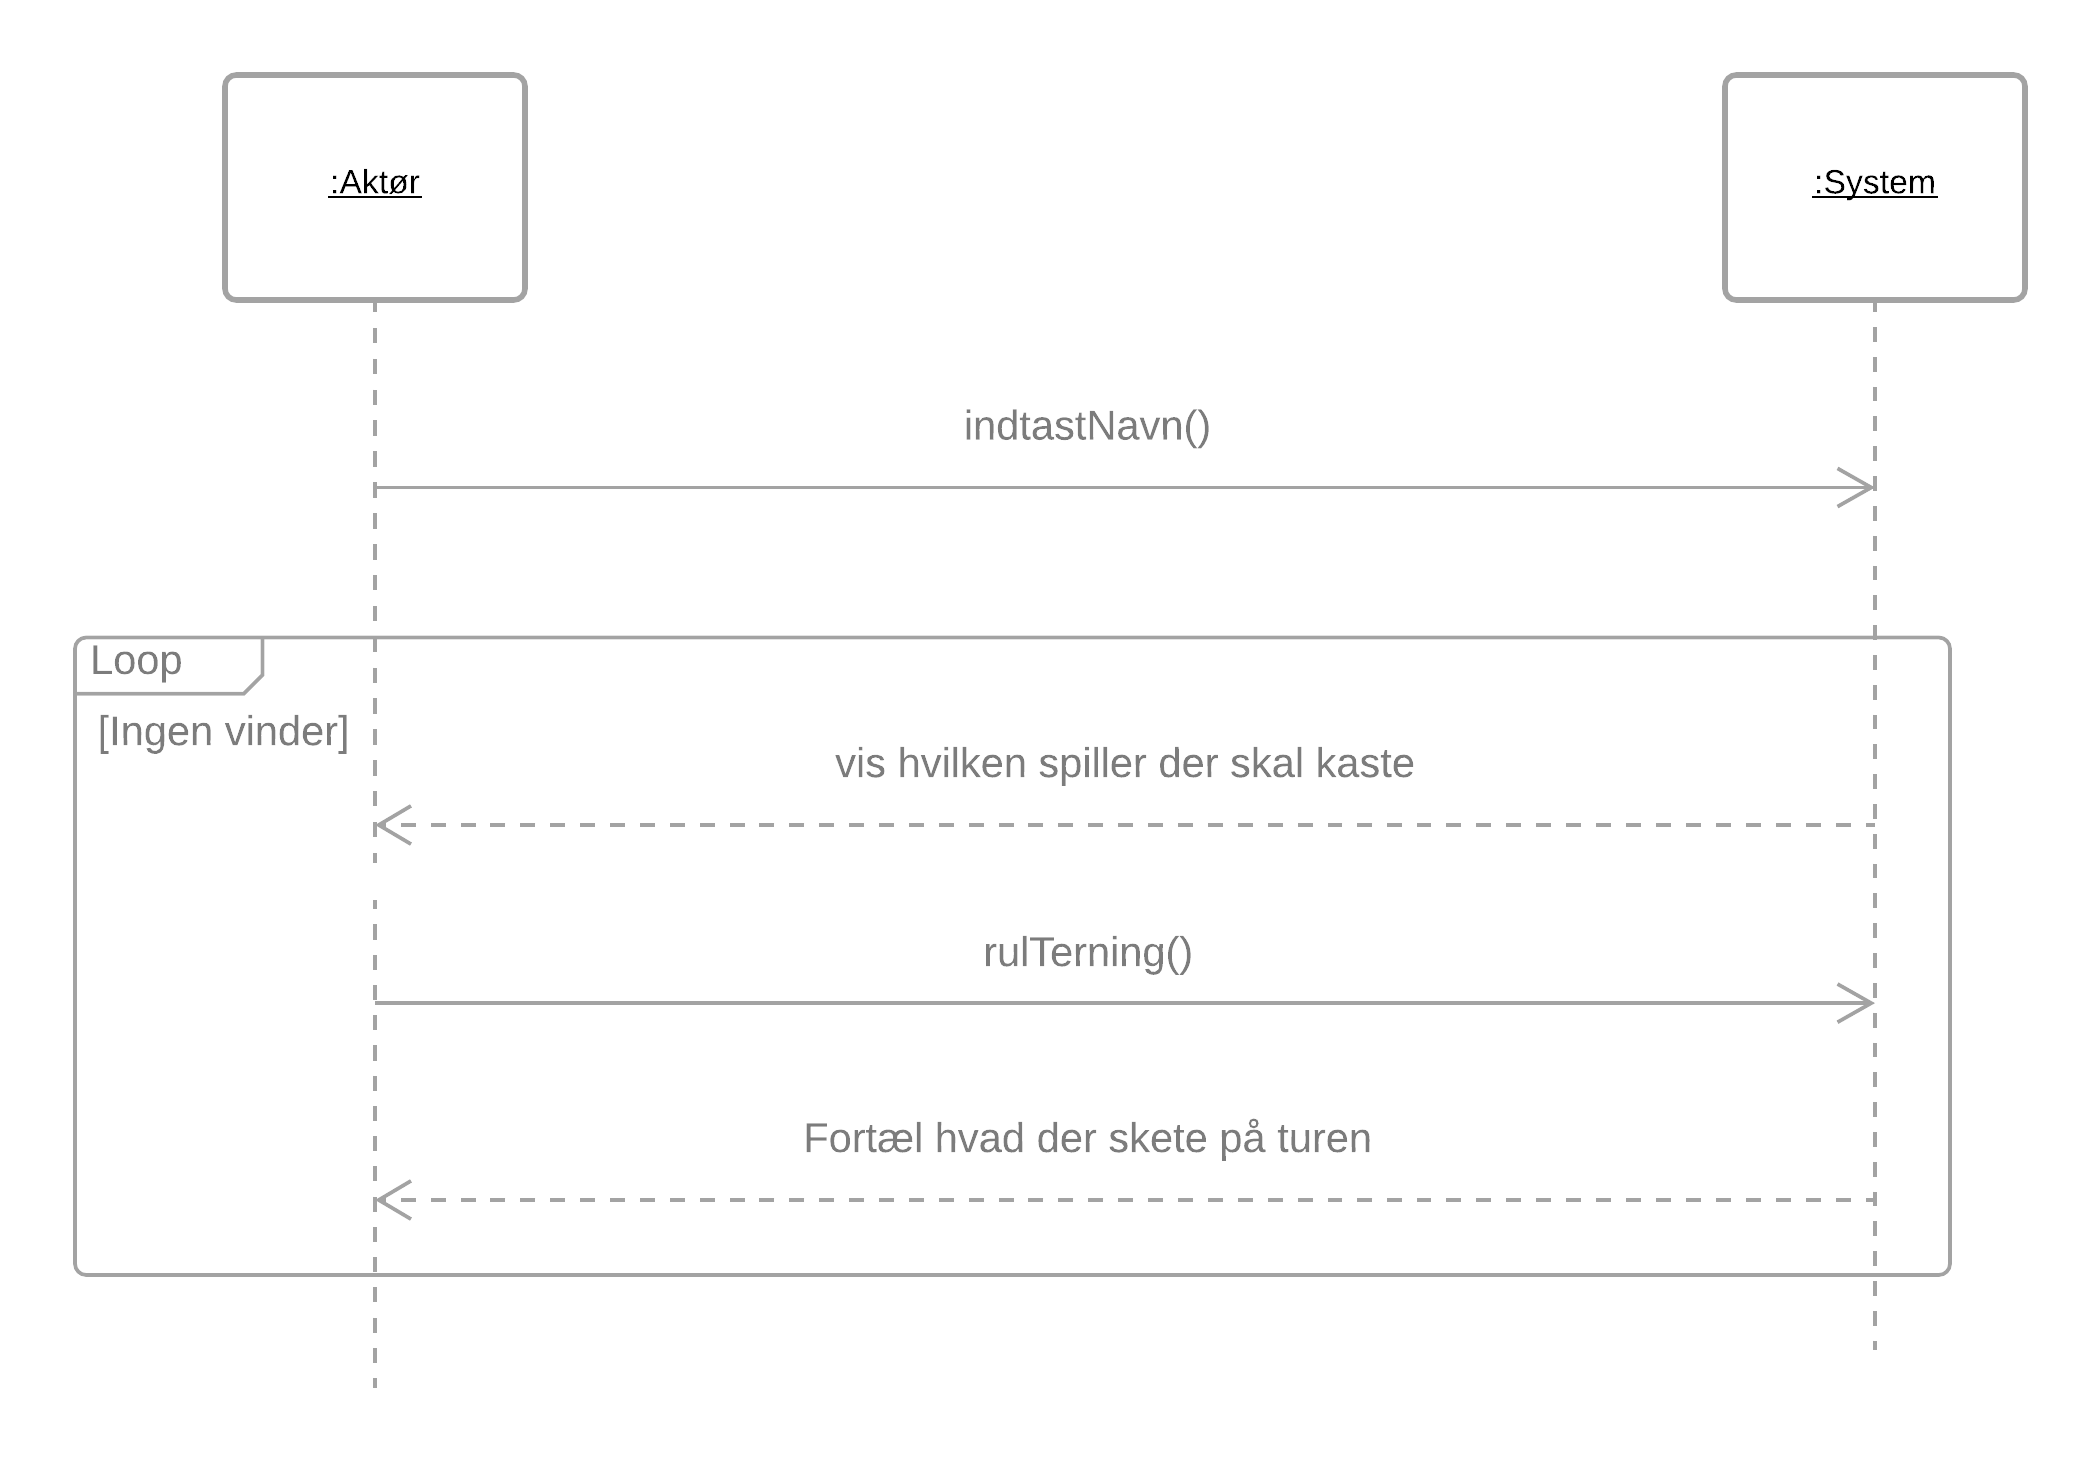
\includegraphics[scale=0.2]{artifacts/SSD.png}
\end{figure}
\newpage
\subsection{Designklassediagram}
\begin{figure}[h!]
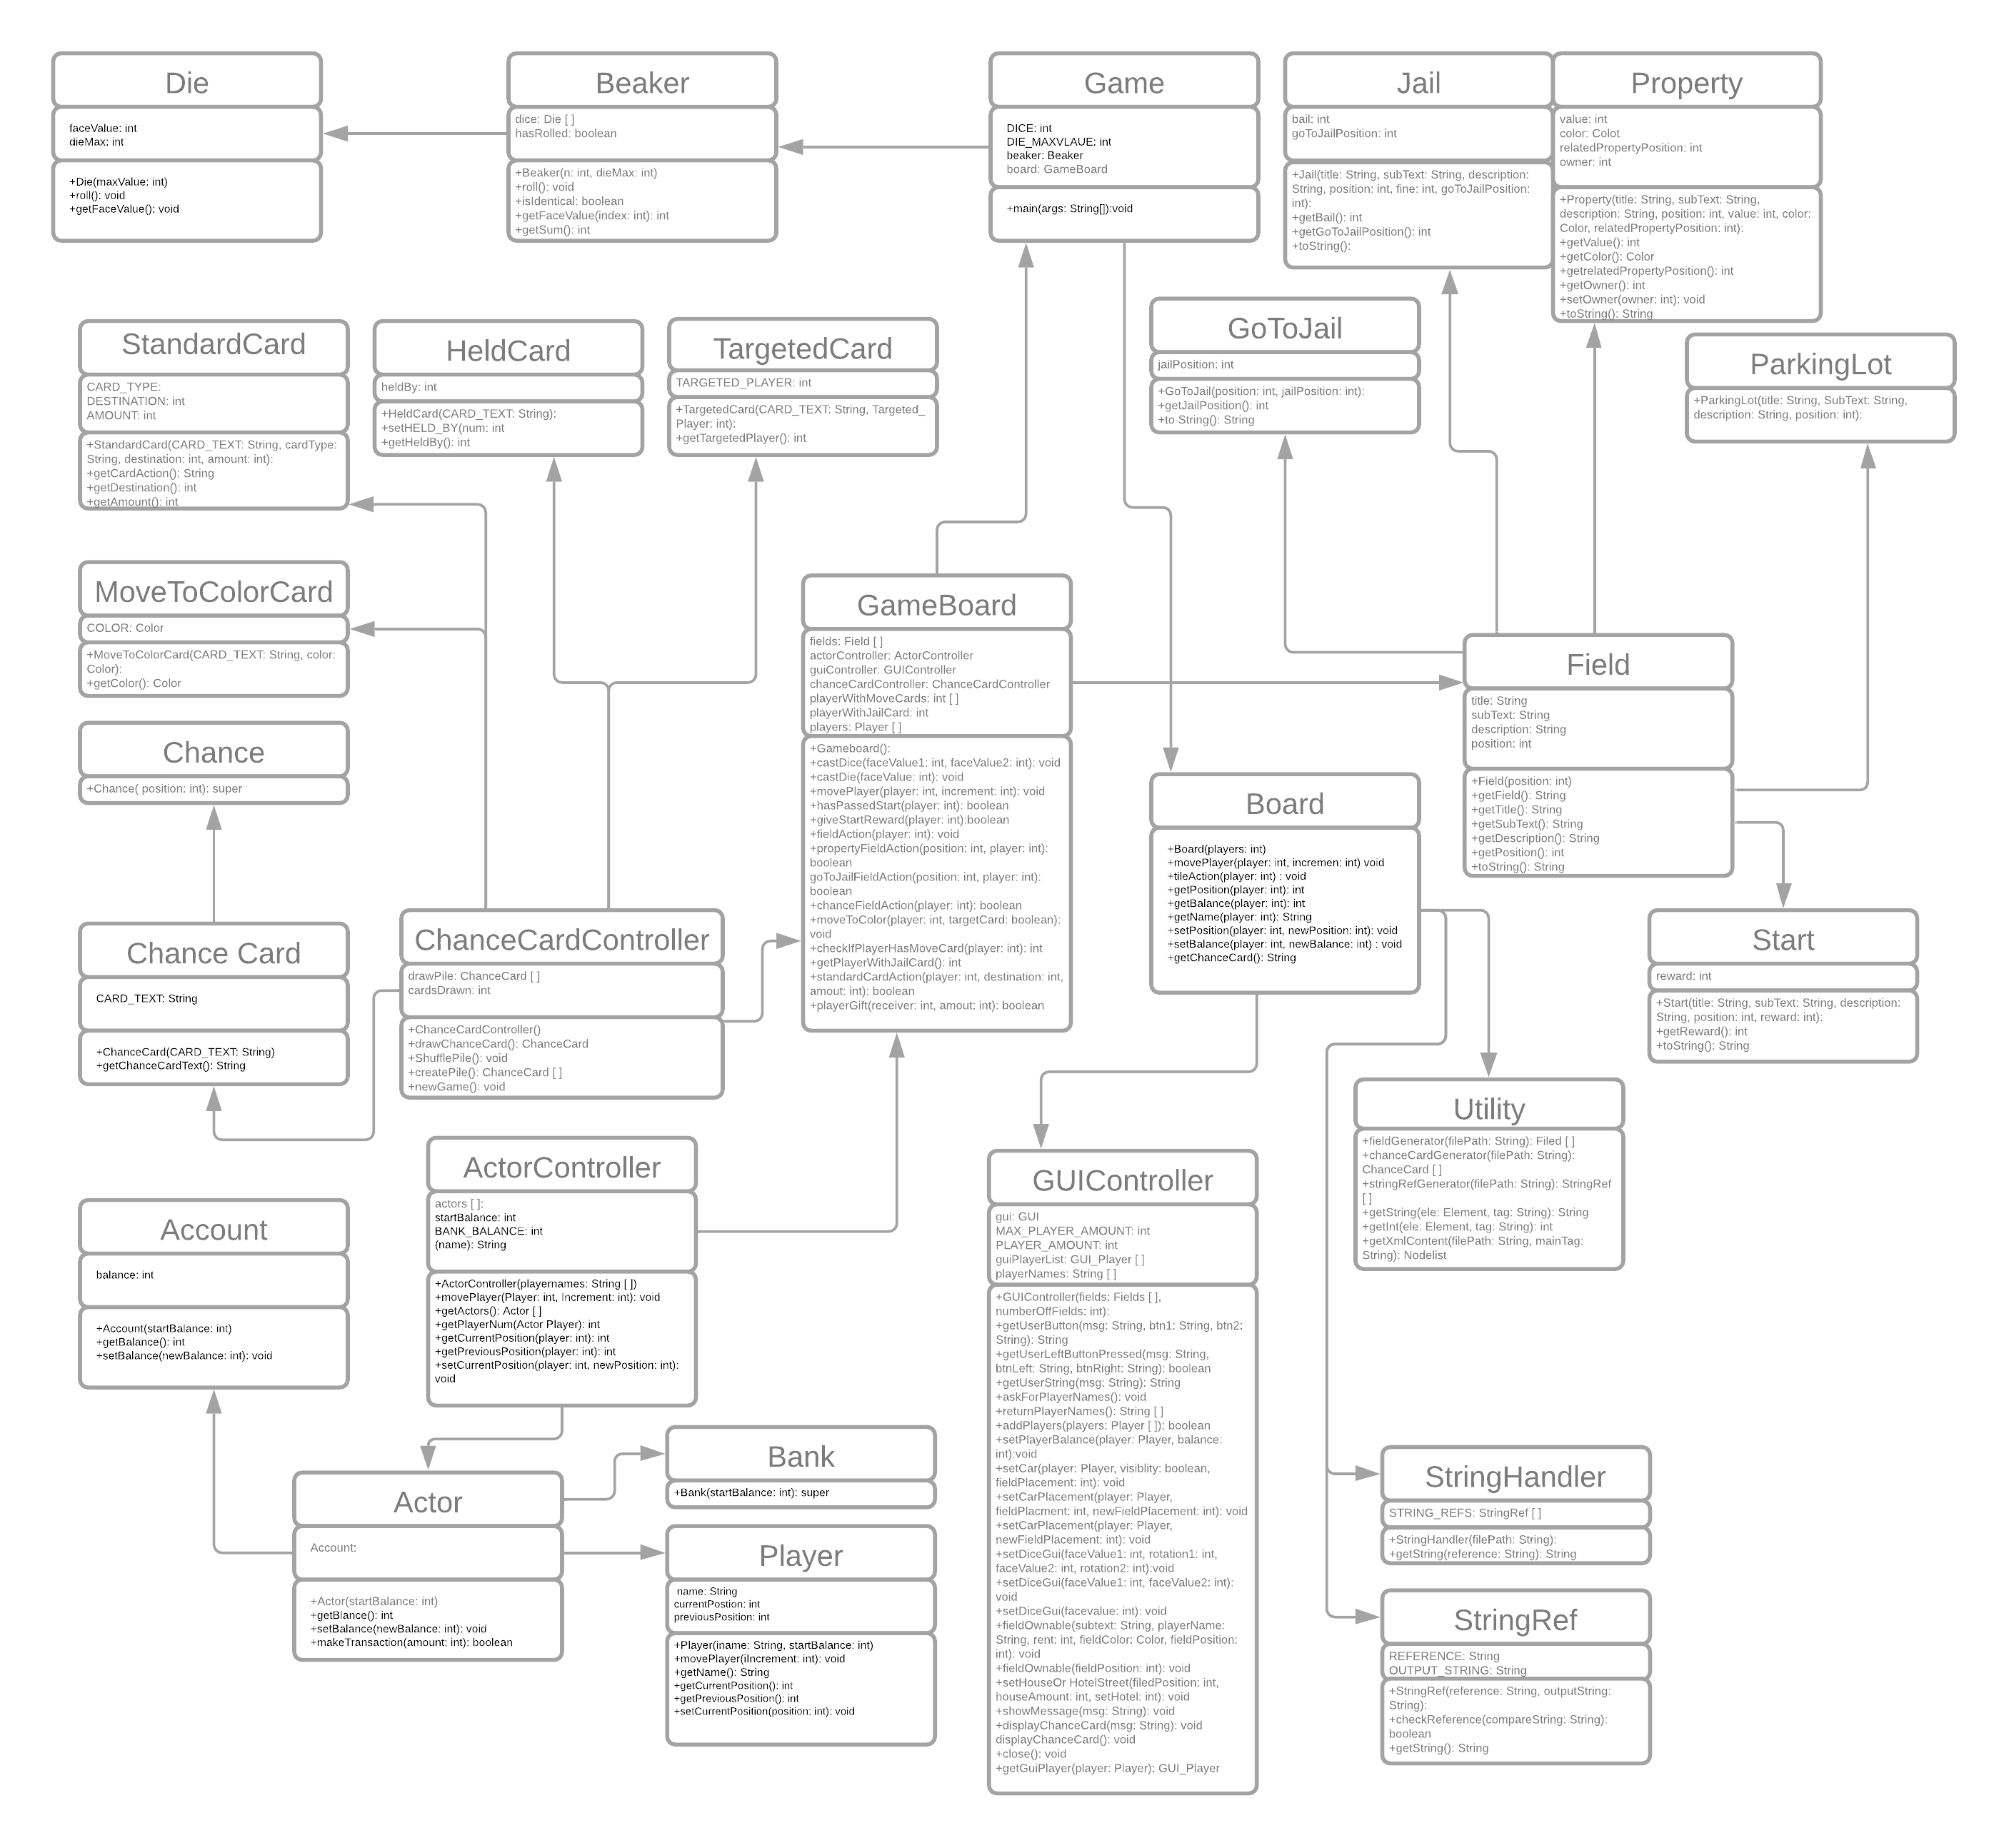
\includegraphics[scale=0.16]{artifacts/DCD.png}
\end{figure}